% Introduction (v2, probe framing). Every number is a \res key.
\section{Introduction}
\label{sec:intro}

A reader consulting a character wiki midway through a series may encounter a later identity,
marriage or death while seeking a reminder of events already read. A reader who has finished
\emph{Anne of Avonlea}, the second book of L.~M.~Montgomery's Anne series, may learn from
Anne Shirley's whole-series page about her marriage to Gilbert Blythe in book four
(Figure~\ref{fig:overview}).\footnote{Examples in this paper reveal plot points of the
series.} A useful reference must respect the reader's progress: at cutoff $t$, every
statement should be established by the first $t$ volumes.

% The overview comes first in the source so that it can take the top of page 2.
\begin{figure*}[t]
\centering
% The teaser has no editable source. f0-teaser-v2.pdf is f0-teaser.pdf with its right-hand
% heading (``Our solution: ...'') and its badge (``No spoilers'') removed from the text layer
% (scripts/papers/redact_teaser_v2.py); both are re-lettered here. Coordinates are fractions
% of the image.
\begin{tikzpicture}
\node[anchor=south west, inner sep=0] (img) at (0,0)
  {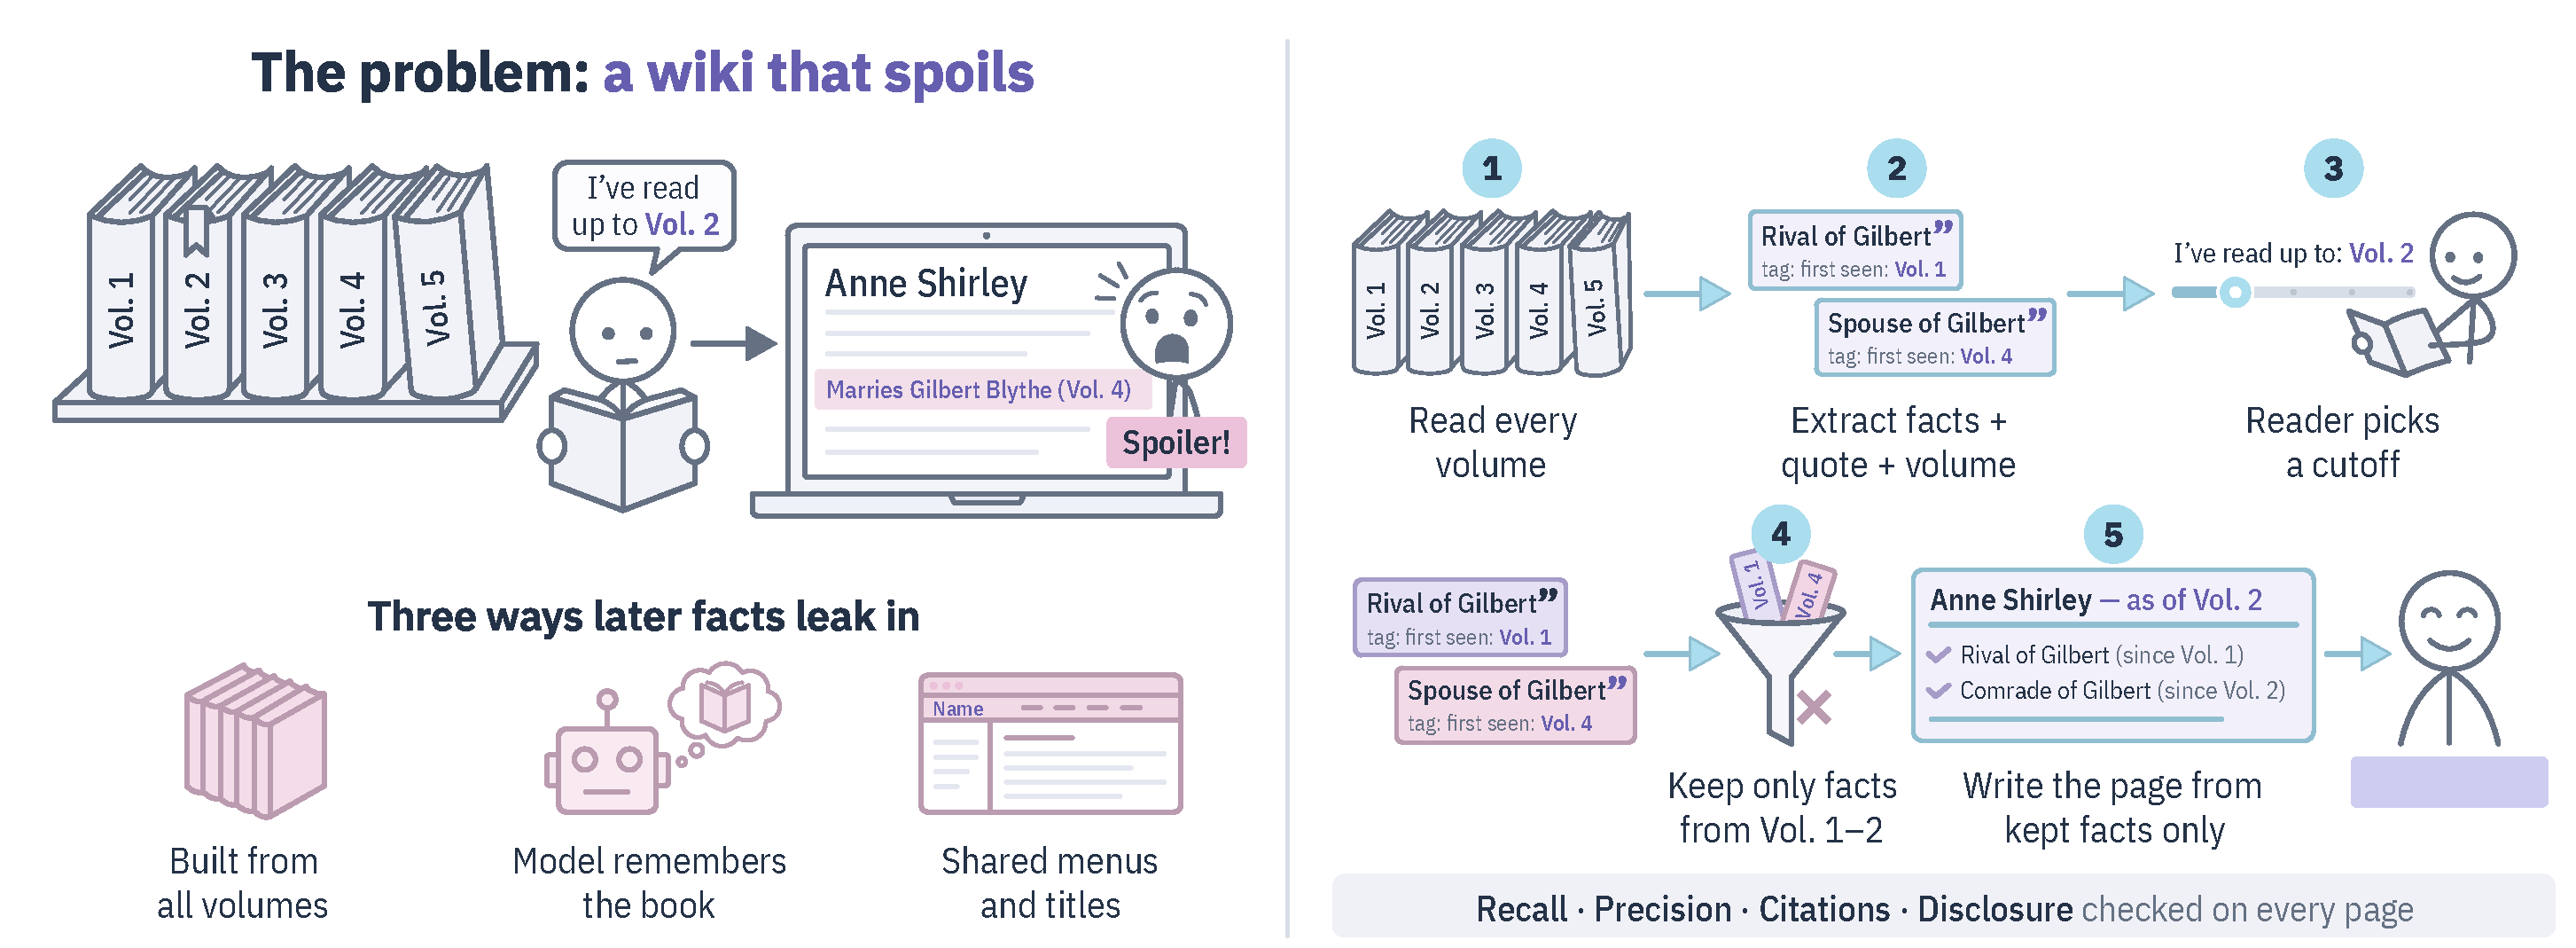
\includegraphics[width=\textwidth]{figures/f0-teaser-v2.pdf}};
\begin{scope}[x={(img.south east)}, y={(img.north west)}]
  \node[font=\sffamily\bfseries\small, text=nwink] at (0.76,0.921)
    {The design under test: \textcolor{nwaccent}{filter, then generate}};
  \node[anchor=north, fill=nwlavender, rounded corners=1pt, inner sep=1.5pt, align=center,
        minimum width=0.08\textwidth, text=nwink,
        font=\sffamily\bfseries\fontsize{5.5}{6}\selectfont] at (0.946,0.207)
    {Cutoff-filtered\\page};
\end{scope}
\end{tikzpicture}
\caption{Overview. Left: a whole-series wiki reveals Anne's marriage to Gilbert (volume~4)
to a reader at volume~2. Later information can enter through a full-series index, generator
memory or surfaces shared across cutoffs. Right: the filter-before-generate design that
\sys implements and this paper probes.}
\label{fig:overview}
\end{figure*}

The natural engineering answer is structural. Decompose the text into a graph of claims,
date each claim by the volume of its evidence, and generate each page from the claims
dated no later than the cutoff, in the manner of graph-based retrieval-augmented generation
\citep{edge2024graphrag,guo2024lightrag}. The boundary is then enforced by data, not by an
instruction to the generator, and one build serves every cutoff. This paper asks what
that decomposition gains and what it costs.

We instrument this design rather than advocate for it. \sys is an \emph{analytical probe}:
it adds verbatim-evidence gates, a claim verifier and logged model calls, which lets us
trace individual errors to the stage that produced them, and it is placed among systems that
differ in what the generator can access and in how pages are written (Figure~\ref{fig:systems}).

Such a comparison is interpretable only if scores reflect reading: given only a title and
a character name, the generator recovers \respt{M1-anne-avg-X1} of the eligible gold
facts. We therefore pair every measurement with a \emph{renamed-text control}: a
\emph{treated} copy of the series renames characters and places and paraphrases nearly
every paragraph, keeping paragraph identifiers so that gold facts and citations stay aligned.
Closed-book recall falls to \respt{M1-annedecon-avg-X1}, while systems given text largely
keep theirs (Section~\ref{sec:results-decon}).

Headline means rank \sys below prompting with the text read so far
(Table~\ref{tab:decon}) and hide both sides of the trade-off. Pages rendered from
accumulated claims, rather than rewritten at each cutoff under a length budget,
\emph{gain}:
\begin{itemize}[leftmargin=*,itemsep=0pt,topsep=2pt]
  \item \textbf{Growing coverage.} In an exploratory split, the highest recall on the
    most-documented characters (\respt{CEN-annedecon-B5} on treated text; long context
    \respt{CEN-annedecon-B1}), rising with the prefix (Section~\ref{sec:results-gains}).
  \item \textbf{Stable pages.} One conveyed fact lost at the next cutoff per text; other
    systems lose \res{DROP-anne-B2} to \res{DROP-annedecon-B2}.
  \item \textbf{Breadth.} A mean of \res{ND-anne-avg-B5} distinct assertions per cutoff from
    one build, against at most \res{ND-anne-avg-B1} for the comparison systems.
\end{itemize}
Replacing the passage with a claim \emph{costs}: each failure below rests on evidence the
cutoff permits, so the volume filter passes it:
\begin{itemize}[leftmargin=*,itemsep=0pt,topsep=2pt]
  \item \textbf{Modality collapse.} A neighbor's prediction that two characters will marry
    is stored as a presumed marriage and rendered as a spouse relation two volumes before
    the wedding (Section~\ref{sec:results-main}).
  \item \textbf{Identity dependence.} Entities resolved over the whole series give early
    pages names and groupings that prefix-built indexes do not reproduce
    (\res{ID-anne-t1-rate} of character pages at $t=1$, \respt{ID-anne-strict-t1} regrouped
    or absent; Section~\ref{sec:results-scope}).
  \item \textbf{Context collapse.} Statements that are true in isolation become unsupported
    on the page where the graph places them (Section~\ref{sec:results-quality}).
\end{itemize}
Prefix-bounded systems that keep the passage in front of the generator, with its speaker
and mood intact, disclosed no assessed later fact. Selection and publication contribute to
the costs: on the original text a baseline that selects facts and evidence from the same
graph is the most precise and best cited (\respt{M3-anne-avg-B4}, \respt{M8-anne-avg-B4}). The control also exposes what the
original text hides: the marriage above appears only on treated text, and an instruction
to withhold later volumes discloses \res{M4U-annedecon-X2} unique later facts on treated
text, against \res{M4U-anne-X2} on the original.

Prior work bounds dialogue or answers in time \citep{ahn2024timechara,huang2025living}.
We study a linked reference artifact at every cutoff:
\begin{itemize}[leftmargin=*,itemsep=0pt,topsep=2pt]
  \item \textbf{A probe study of structural decomposition} under a reading cutoff,
    separating its gains from failures that a volume filter cannot detect
    (Sections~\ref{sec:method}, \ref{sec:results}).
  \item \textbf{A paired renamed-text control} as evaluation methodology: seven systems
    rebuilt on aligned treated text with unchanged code, prompts and gold facts, and
    recognition measured separately from recall (Section~\ref{sec:results-decon}).
  \item \textbf{A task, threat model and artifact-level protocol} for cutoff-bounded
    reference generation, with \res{T1-anne-gold-t5} gold facts dated by reveal volume
    (Sections~\ref{sec:task}, \ref{sec:setup}; Appendix~\ref{app:corpus}).
\end{itemize}
